\begin{frame}{2.3.7 スチューデントのt分布}
 \begin{itemize}
  \item これまでに、ガウス分布の精度パラメータの共役事前分布がガンマ分布となることを見てきた
  \item 1変数のガウス分布$\mathcal{N}(x|\mu, \tau^{-1})$において、ガンマ分布${\rm Gam}(\tau|a,b)$を精度の事前分布とし、そこから精度を積分消去し、$z=\tau[b+(x-\mu)^2/2]$の変数の置換を用いると、$x$の周辺分布は次式となる
        \begin{eqnarray}
         && p(x|\mu,a,b) \nonumber \\
         &=& \int_0^\infty \mathcal{N}(x|\mu,\tau^{-1}){\rm Gam}(\tau|a,b)d\tau\label{133939_19Nov14} \\
         % &= & \int_{0}^{\infty}\frac{b^ae^{-b\tau}\tau^{a-1}}{\Gamma(a)}(\frac{\tau}{2\pi})^{1/2}\exp\{-\frac{\tau}{2}(x-\mu)^2\}d\tau \nonumber\\
         &= & \frac{b^a}{\Gamma(a)}\left(\frac{1}{2\pi}\right)^{1/2}\left[b+\frac{(x-\mu)^2}{2}\right]^{-a-1/2}\!\!\!\!\!\!\Gamma(a+1/2)
        \end{eqnarray}
 \end{itemize}
\end{frame}

\begin{frame}{スチューデントのt分布}
 \begin{itemize}
  \item 慣例により、$\nu=2a$と$\lambda=a/b$のパラメータを新たに定義すると、\alert{スチューデントのt分布}が得られる
        \begin{equation}
         {\rm St}(x|\mu,\lambda,\nu) = \frac{\Gamma(\nu/2+1/2)}{\Gamma(\nu/2)}\left(\frac{\lambda}{\pi\nu}\right)^{1/2}\left[1+\frac{\lambda(x-\mu)^2}{\nu}\right]^{-\nu/2-1/2}
        \end{equation}
        \begin{itemize}
         \item パラメータ$\lambda$はt分布の精度とも呼ばれるが、必ずしも分散の逆数とは限らない
         \item パラメータ$\nu=1$ではコーシー分布、$\nu\rightarrow\infty$では平均が$\mu$で精度が$\lambda$のガウス分布になる
        \end{itemize}
  \item 式(\ref{133939_19Nov14})より、スチューデントのt分布は、平均は同じだが精度は異なるようなガウス分布を無限個足し合わせたものであることがわかる
        \begin{itemize}
         \item ガウス分布の無限混合分布(詳細は2.3.9節)
        \end{itemize}
 \end{itemize}
\end{frame}

%図を挿入するときは.epsファイルを使う
%jpgなどだと、画面外に画像が配置される(意味不明)
% .epsは神。
\begin{frame}{スチューデントのt分布}
 \begin{center}
  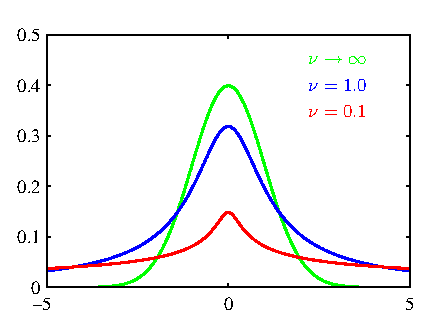
\includegraphics[scale=1.0]{./figure/Figure2.15.eps}
 \end{center}
\end{frame}

\begin{frame}{頑健性と回帰問題}
 \begin{itemize}
  \item スチューデントのt分布はガウス分布より一般に「すそ」が長く、\alert{頑健性}を持つ
        \begin{itemize}
         \item 外れ値となっている少数のデータ点があっても、ガウス分布よりは影響されにくい
        \end{itemize}
  % \item 外れ値は、実際にデータを生成する分布のすそが大きい場合や、単純なラベル付けの誤りなどにあるように、実際の問題ではよく生じる
  % \item 頑健性は回帰問題でも重要な性質である
  % \item 回帰での最小二乗法は、条件付きガウス分布の下での最尤推定に相当するので、頑健ではない
  % \item そこで、すその重い分布に基づく回帰モデルを用いる
 \end{itemize}
        \begin{tabular}[tb]{cc}
         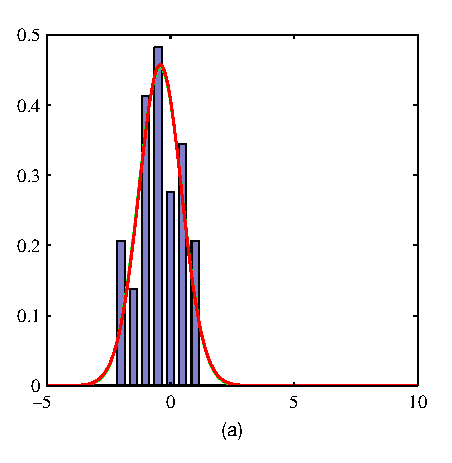
\includegraphics[width=0.5\textwidth]{./figure/Figure2.16a.eps}
         &
         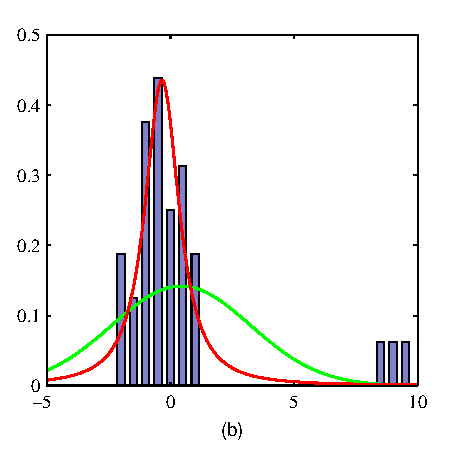
\includegraphics[width=0.5\textwidth]{./figure/Figure2.16b.eps}
        \end{tabular}
\end{frame}

\begin{frame}{多変量のスチューデントt分布}
 \begin{itemize}
  \item 式(\ref{133939_19Nov14})に戻って、パラメータを$\nu=2a,\lambda=a/b,$および$\eta=\tau b/a$と置き換えると、t分布は次の形に書ける
        \begin{equation}
         {\rm St}(x|\mu,\lambda,\nu) = \int_{0}^{\infty}\mathcal{N}(x|\mu, (\eta\lambda)^{-1}){\rm Gam}(\eta|\nu/2,\nu/2)d\eta
        \end{equation}
  \item これは多変量ガウス分布の場合に一般化でき、多変量スチューデントt分布に相当するものが次式で得られる
        \begin{equation}
         {\rm St}(\bm{x}|\bm{\mu},\bm{\Lambda},\nu) = \int_{0}^{\infty}\mathcal{N}(\bm{x}|\bm{\mu}, (\eta\bm{\Lambda})^{-1}){\rm Gam}(\eta|\nu/2,\nu/2)d\eta
        \end{equation}
 \end{itemize}
\end{frame}

\begin{frame}{多変量のスチューデントt分布}
 \begin{itemize}
  \item 1変数の場合と同じように、積分を計算すると
        \begin{eqnarray}
         {\rm St}(\bm{x}|\bm{\mu},\bm{\Lambda},\nu) &=& \frac{\Gamma(D/2+\nu/2)}{\Gamma(\nu/2)}\frac{|\bm{\Lambda}|^{1/2}}{(\pi\nu)^{D/2}}\left[1+\frac{\Delta^2}{\nu}\right]^{-D/2-\nu/2} \\
         \Delta^2&= & (\bm{x}-\bm{\mu})^{\mathrm{T}}\bm{\Lambda}(\bm{x}-\bm{\mu})
        \end{eqnarray}
        を得る
  \item これはスチューデントt分布の多変量型で、1変数の結果に対応した、次の性質を満たす
        \begin{align}
         \mathbb{E}[\bm{x}]&=& \bm{\mu}&, && \text{$\nu>1$のとき}\\
         {\rm cov}[\bm{x}]&=&\frac{\nu}{(\nu-2)}\bm{\Lambda}^{-1}&,  &&\text{$\nu>2$のとき}\\
         {\rm mode}[\bm{x}]& =& \bm{\mu} &&&
        \end{align}
 \end{itemize}
\end{frame}
